\section{Software Implementation}
\label{sec:implementation}

OpenRAM is implemented using object-oriented data structures in the
Python programming language. The top-level executable is
\verb|openram.py| which parses input arguments, creates the memory and
saves the output.


\subsection{Design Hierarchy}
\label{sec:design}

All modules in OpenRAM are derived from the \verb|design| class in
\verb|design.py|. The design class is a data structure that consists
of a spice netlist, a layout, and a name. The spice netlist
capabilities are inherited from the \verb|hierarchy_spice| class while
the layout capabilities are inherited from the \verb|hierarchy_layout|
class.  The only additional function in design.py is \verb|DRC_LVS()|,
which performs a DRC/LVS check on the module.


\begin{figure}[htb]
\centering
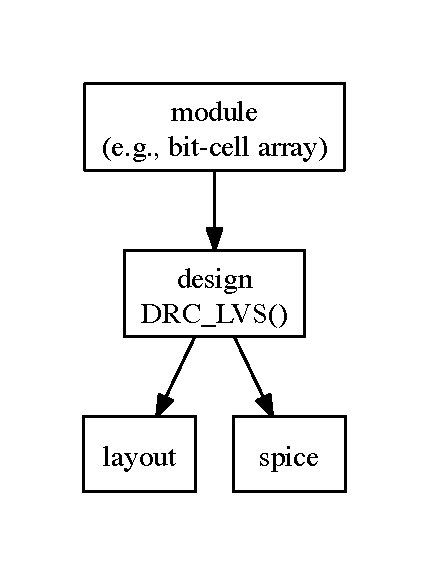
\includegraphics[width=10cm]{./figs/class_hierarchy.pdf}
\caption{Class hierarchy}
\label{fig:class_hierarchy}
\end{figure}

\subsubsection{Spice Hierarchy}

The spice hierarchy is stored in the \verb|spice| class in
\verb|hierarchy_spice.py|.  When the design class is initialized for a
module, a data structure for the spice hierarchy is created.  The
spice data stucture name becomes the name of the top-level subcircuit
definition for the module.  The list of pins for the module are added
to the subcircuit definition by using the \verb|add_pin()| function.
The \verb|add_mod()| function adds an instance of a
module/library\_cell/parameterized\_cell as a subcircuit to the
top-level structure.  Each time a sub-module has been added to the
hierarchy, the pins of the sub-module must be connected using the
\verb|connect_pins()| function.  It is important to note that the pins
must be listed in the same order as they were added to the submodule.
Also, an assertion error will occur if there is a mismatch in the
number of net connections.  The \verb|spice| class also contains
functions for reading or writing spice files:
\begin{itemize}
\item \verb|sp_read():| this function is used to read in spice
  netlists and parse the inputs defined by the ``subckt'' definition.
\item \verb|sp_write():| this function creates an empty spice file in
  write mode and calls \verb|sp_write_file()|.
\item \verb|sp_write_file():| this function recursively writes the
  modules and sub-modules from the data structure into the spice file
  created by \verb|sp_write()|.
\end{itemize}

\subsubsection{Layout Hierarchy}

The layout hierarchy is stroed in the \verb|layout| class in
\verb|hierarchy_layout.py|.  When the design class is initialized for
a module, a data structure for the layout hierarchy is created.  The
layout data structure has two main components: a structure for the
instances of sub-modules contained in the layout, and a structure for
the objects (such as shapes, labels, etc...) contained in the layout.
The functions included in the \verb|layout| class are:
\begin{itemize}
\item \verb|def add_inst(self,name,mod,offset,mirror):| adds an
  instance of a physical layout (library cell, module, or
  parameterized cell) to the module. The input parameters are :
  \begin{description}
  \item[name] - name for the instance.
  \item[mod] - the associated spice module.
  \item[offset] - the x-y coordinates, in microns, where the instance
    should be placed in the layout.
  \item[mirror] - mirror or rotate the instance before it is added to
    the layout.  Accepted values for mirror are:
    \verb|"R0", "R90", "R180", "R270"|  $^\ast$Currently, only ``R0'' works.\\
    \verb|"MX" or "x", "MY" or "y", "XY" or "xy"| (``xy'' is
    equivalent to ``R180'')
  \end{description}
\item \verb|add_rect(self,layerNumber,offset,width,height):| adds a
  rectangle to the module's layout. The inputs are:
  \begin{description}
  \item[layernumber] - the layer that the rectangle is to be drawn in.
  \item[offset] - the x-y coordinates, in microns, where the
    rectangle's origin will be placed in the layout.
  \item[width] - the width of the rectangle, can be positive or
    negative value.
  \item[height] - the height of the rectangle, can be positive or
    negative value.
  \end{description}
\item \verb|add_label(self,text,layerNumber,offset,zoom):| adds a
  label to the layout. The inputs are:
  \begin{description}
  \item[text] - the text for the label
  \item[layernumber] - the layer that the label is to be drawn in .
  \item[offset] - the x-y coordinates, in microns, where the label
    will be placed in the layout.
  \item[zoom] - magnification of the label (ex: ``1e9'').
  \end{description}
\item \verb|add_path(self,layerNumber,coordinates,width):| this
  function is under construction...
\item \verb|gds_read():| reads in a GDSII file and creates a
  \verb|VlsiLayout()| class for it.
\item \verb|gds_write():| writes the entire GDS of the object to a
  file by gdsMill \verb|vlsiLayout()| class and calling the
  \verb|gds2writer()| (see Sections~\ref{sec:vlsilayout}
  and~\ref{sec:gdsmill}.
\item \verb|gds_write_file():| recursively the instances and objects
  in layout data structure to the gds file.
\item \verb|pdf_write():| this function is under construction...
\end{itemize}


\subsection{Creating a New Design Module}
\label{sec:new_design}

Each module in the SRAM is its own Python class, which contains a
design class, or data structure, for the layout and spice.  The
\verb|design| class (\verb|design.py|) is initialized within the
module class, subsequently creating separate data structurse to hold
the layout (\verb|hierarchy_layout|) and spice
(\verb|hierarchy_spice|) information.  By having a class for each
module, it is very easy to instatiate instances of the modules in any
level of the hierarchy.  Follow these guidelines when creating a new
module:


\begin{itemize}
\item Derive your class from the design module:
\begin{verbatim}
class bitcell_array(design.design):
\end{verbatim}
\item Always use the python constructor \verb|__init__| method so that
  your class is initialized when an object of the module is
  instatiated. The module parameters should also be declared:
\begin{verbatim}
def __init__(self, cols, rows): 
\end{verbatim}
\item In the constructor, call the base class constructor with the
  name such as:
\begin{verbatim}
design.design.__init__(self,"bitcell_array")
\end{verbatim}
\item Add the pins that will be used in the spice netlist for your
  module using the \verb|add_pin()| function from the
  \verb|hierarchy_spice| class.
\begin{verbatim}
self.add_pin("vdd")
\end{verbatim}
\item Create an instance of the module/library\_cell/parameterized
  cell that you want to add to your module:
\begin{verbatim}
cell=bitcell.bitcell(cell_6t)
\end{verbatim}
\item Add the subckt/submodule instance to the spice hierarchy using
  the \verb|add_mod()| function from the \verb|hierarchy_spice| class:
\begin{verbatim}
self.add_mod(cell)
\end{verbatim}
\item Add layout instance into your module's layout hierarchy using
  the \verb|add_instance|() function, which takes a name, mod, offset,
  and mirror as inputs:
\begin{verbatim}
self.add_inst(name=name,mod=cell,offset=[x_off,y_off],mirror=x)
\end{verbatim}
\item Connect the pins of the instance that was just added by using
  the \verb|connect_pins| function from the \verb|hierarchy_spice|
  class:
\begin{verbatim}
self.connect_inst([BL[%d]%col, BR[%d]%col, WL[%d]%row, gnd, vdd]).  
\end{verbatim}	
  The pins must be listed in the same order as they were added to the
  submodule.  Also, an assertion error will occur if there is a
  mismatch in the number of net connections.
\item Do whatever else needs to be done. Add rectangles for
  power/ground rails or routing, add labels, etc...
\item Every module needs to have ``self'' height and width variable
  that can be accessed from outside of the module class.  These
  paramaters are commonly used for placing instances modules in a
  layout.  For library cells, the \verb|self.width| and
  \verb|self.height| variables are automatically parsed from the GDSII
  layout using the \verb|cell_size()| function in \verb|vlsi_layout|.
  Users must define the width and height of dynamically generated
  designs.
\item Add a call to the \verb|DRC_LVS()| function.
\end{itemize}

\subsection{GDSII Files and GdsMill)}
\label{sec:gds}

GDSII is the standard file used in indusrty to store the layout
information of an integrated circuit. The GDSII file is a stream file
that consists of records and data types that hold the data for the
various instances, shapes, labels, etc.. in the layout. In OpenRAM, we
utlize a nifty tool, called gdsMill, to read, write, and manipulate
GDSII files.  GdsMill was developed by Michael Wieckowski at the
University of Michigan.

\subsubsection{GDSII File Format}
\label{sec:format}

The format of gds file contains several parts, as it could be shown in
Figure~\ref{fig:gds_file}.

\begin{figure}[htb]
\centering
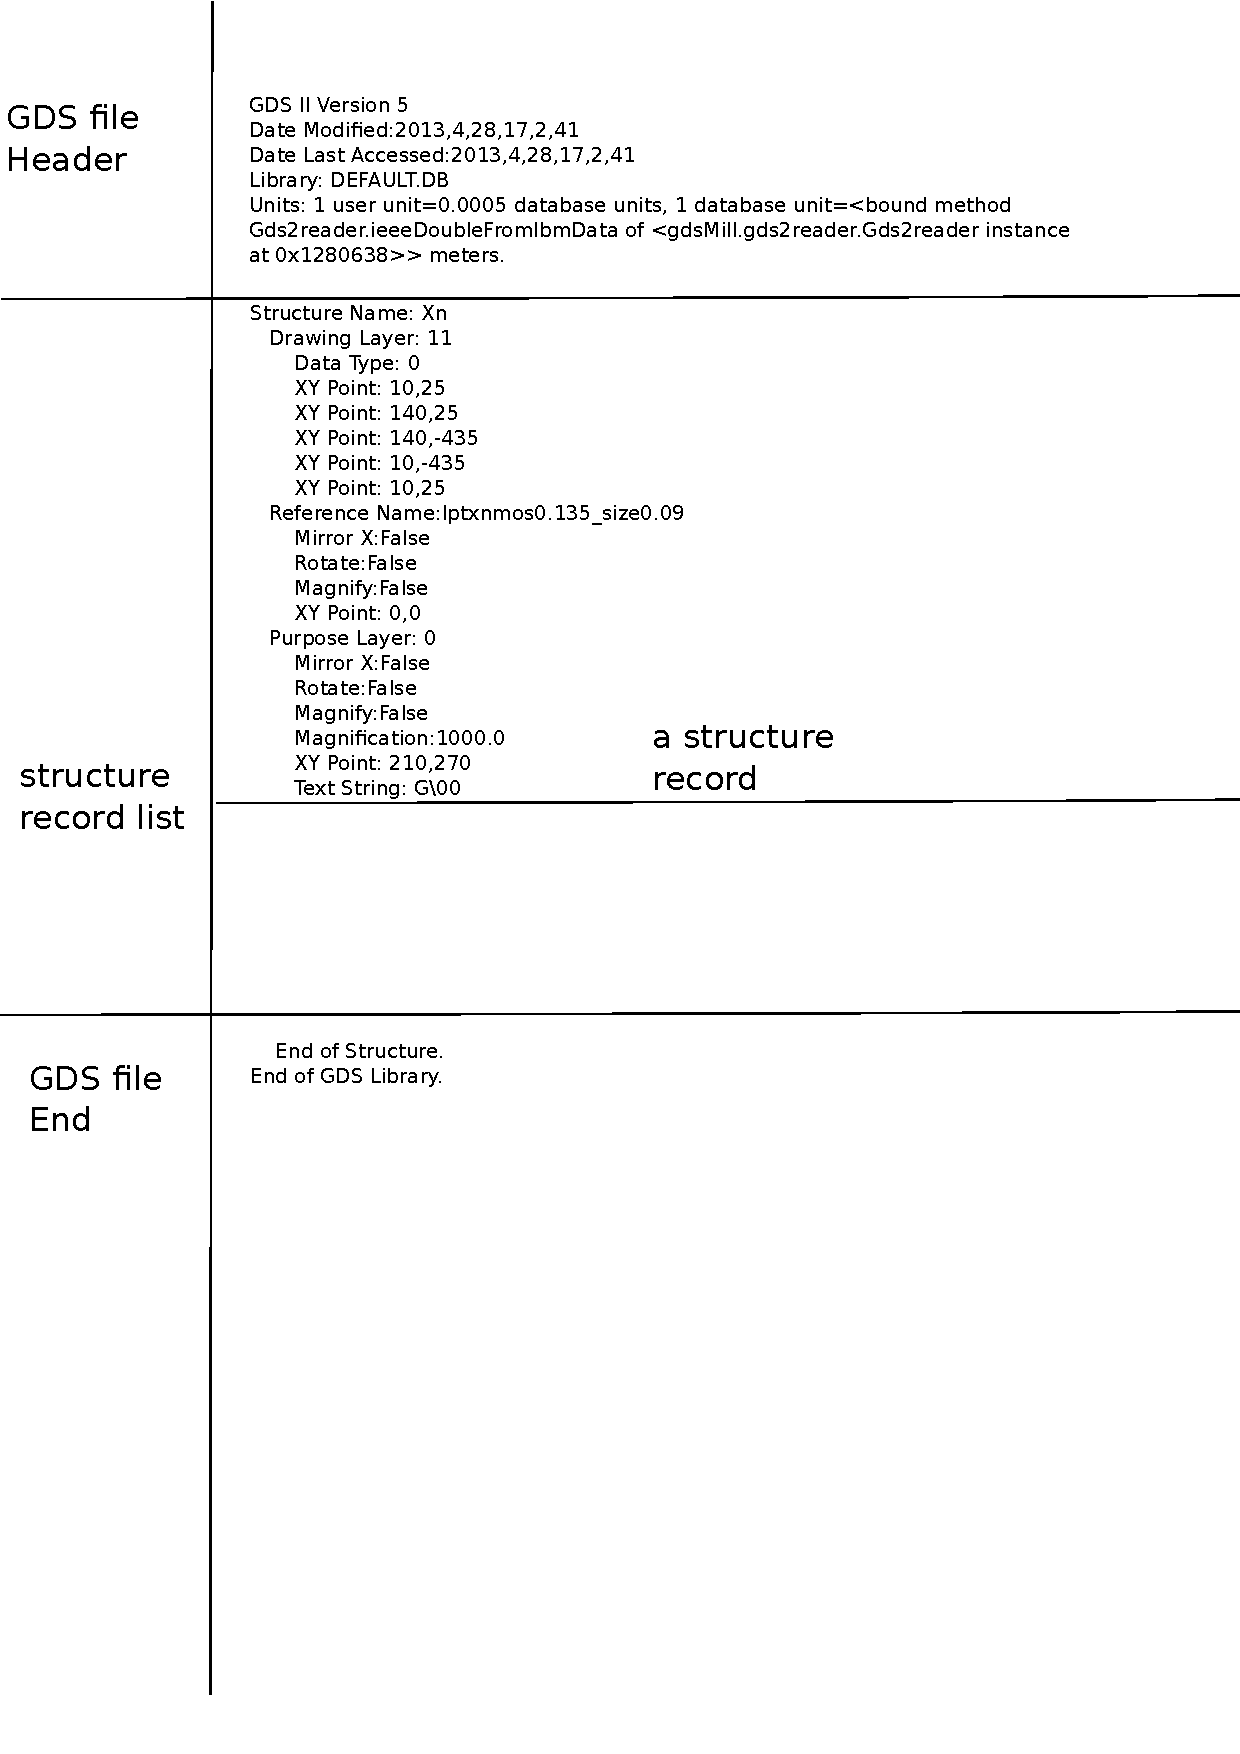
\includegraphics[width=10cm]{./figs/gds_file}
\caption{example of a GDSII file}
\label{fig:gds_file}
\end{figure}

The first part is the gds file header, which the contains GDSII
version number, date modified, date last accessed, library, user
units, and database units.

The second part is the list of structures.  These structures contain
geometries or references to other structures of the layout in
heirarchical form.  Within a structure there are several kinds of
records:

\begin{itemize}
\item Rectangle - basic geometry unit in a design, represent one layer
  of material in a circuit(i.e. a metal pin). Five coordinates and
  layer number are stored in rectangle record.
\item Structure Reference - a structure that is used in this
  structure. The information about this reference will be used store
  as a structure in the same gds file.
\item Text - a text record used for labels.
\item Path - used to represent a wire.
\item Boundary - defines a filled polygon.
\item Array Reference - specifies an array of structure instances
\item Node - Electrical nets may be specified with the NODE record
\end{itemize}

The last part is the tail of the GDSII file which ends the GDS
Library.

\fixme{Provide a link to the complete GDSII specification.}

\subsubsection{GdsMill}
\label{sec:gdsmill}

As previously stated, GdsMill is a set of scripts that can be used to read, write, and manipulate GDSII files. 

\paragraph{The gds2\_reader and gds2\_writer:}

In GdsMill, the \verb|gds2_reader| and \verb|gds2_writer| classes contain the various functions used to convert data between GDSII files and the \verb|vlsilayout| class. These classes process the data by iterating through every record in the GDS structures and check or write every data record. The record type (see Section~\ref{sec:format}),is tracked and identified using flags.

\fixme{Do we need more information of these classes, or should we just point to the GdsMill documentation?}

\paragraph{The VlsiLayout Class:}
\label{sec:vlsilayout}

After the \verb|gds2_reader| class reads in the records, the data has to be stored in a
way that can be easily used by our code. Thus, the
\verb|VlsiLayout| class is made to represent the layout.
\verb|VlsiLayout| contains the same information as GDSII file but in a
different way. \verb|VlsiLayout| stores records in data structures, which
are defined in \verb|gdsPrimitives.py|.  Each record type has a corresponding class defined in \verb|gdsPrimitives|.  Thus, a vlsilayout should at least
contains following member data:
\begin{itemize}
\item \verb|self.rootStructureName| - name of the top design.
\item \verb|self.structures| -list of structure that are used in the class. 
\item \verb|self.xyTree| - contains a list of all structure names that appeared in the design. 
\end{itemize}

The \verb|VlsiLayout| class also contains many functions for adding
structures and records to a layout class, but the important and most
useful functions have been aggregated into a wrapper file.  This
wrapper is called \verb|geometry.py| and is located in the
\verb|compiler| directory.

\subsubsection{OpenRAM-GdsMill Interface}
\label{sec:wrapper}

Dynamically generated cells and arrays each need to build a
\verb|VlsiLayout| data structure to represent the hierarchical layout.
This is performed using various functions from the \verb|VlsiLayout|
class in GdsMill, but the GdsMill file is very large and can be
difficult to understand.  To make things easier, OpenRAM has its own
wrapper class called \verb|geometry| in \verb|geometry.py|.  This
wrapper class initializes data structures for the
instances and objects that will be added to the \verb|VlsiLayout|
class.  The functions \verb|add_inst()|, \verb|add_rect()|,
\verb|add_label()| in \verb|hierarchy_layout|, add the structures to
the \verb|geometry| class, which is then written out to a GDSII file
using \verb|VlsiLayout| and the \verb|gds2_writer|.

User included library cells, which should be in gds files, can be used
as dynamically generated cells by using GDSMill.
Cell information such as cell size and pin location can be obtained by using
built in functions in the \verb|VlsiLayout| class.

Cell size can be finded by using the \verb|readLayoutBorder| function of the \verb|VlsiLayout| class.
A boundary layer should be drawn in each library cell to indicate the cell area.
The \verb|readLayoutBorder| function will return the width and height of the boundary.
If a boundary layer do not exist in the layout, then \verb|measureSize| can find the physical 
size cell.
The first method is used as primary method in \verb|auto_Measure_libcell| the lib\_utility.py,
while the second method is used as a back up one.
Each technolgy setup will import this utility function and read the library cell.

Pin location can be find by using the \verb|readPin| function of the \verb|VlsiLayout| class.
The \verb|readPin| function will return the biggest boundary which covers the label and 
is at the same layer as the label is.


\subsection{Technology Directory}
\label{sec:techdir}

The aim of creating technology directory is to make OpenRAM portable
to different technologies. This directory contains all the information
related to the specific process/technology that is being used.  In
OpenRAM, the default technology is FreePDK45, which has it own
technolony directory in the trunk.  The technology-specific directory
should consist of the following:
\begin{itemize}
\item Technology-Specific Parameters - These parameters should include
  layer numbers and any design rules that may be needed for generating
  dynamic designs (DRC rules). The parameters should be added in
  \verb|/techdir/tech/tech.py| and layer map in the \verb|/techdir|.
\item Library Cells - The library cells and corresponding spice
  netlists should be added to the \verb|/gds_lib| and \verb|/sp_lib|
  directories.
\item Portation Functions - Some of the dynamically generated cells
  may need helper functions to deal with technology-specific
  requirements.  Additional, tech-specific, functions should be added
  to the \verb|/techdir|.
\end{itemize}

For more information regarding the technology directory and how to set
one up for a new technology, refer to Section~\ref{sec:porting}

\subsection{DRC/LVS Interface}
\label{sec:drclvs}

Each design class contains a function \verb|DRC_LVS()| that performs both
DRC and LVS on the current design module. This enables bottom-up
correct-by-construction design and easy identification of where errors
occur. It does incur some run-time overhead and can be disabled on
the command line. The \verb|DRC_LVS()| function saves a GDSII file and a Spice
file into a temporary directory and then calls two functions to
perform DRC and LVS that are tool-dependent.

A reference implementation for the DRC and LVS functions are provided
for Cadence Calibre since this is the most common DRC/LVS tool. Each
of these functions generates a batch-mode ``runset'' file which
contains the options to correctly run DRC and LVS. The functions then
parse the batch mode output for any potential errors and returns the
number of errors encountered.

The function \verb|run_drc()| requires a cell name and a GDSII
file. The cell name corresponds to the top level cell in the GDSII
file. It also uses the layer map file for the technology to correctly
import the GDSII file into the Cadence database to perform DRC. The
function returns the number of DRC violations. 

The function \verb|run_lvs()| requires a cell name, a GDSII file, and
a Spice file. Calibre will extract an extracted Spice netlist from the
GDSII file and will then compare this netlist with the OpenRAM Spice
netlist. The function returns the number of uncompared and unmatched
devices/nets in the design.

For both DRC and LVS, the summary file and other report files are left
in the OpenRAM temporary directory after DRC/LVS is run. These report
files can be examined to further understand why errors were
encountered. In addition, by increasing the debug level, the command
line to re-create the DRC/LVS check can be obtained and run manually.





